\documentclass[]{article}
\usepackage{lmodern}
\usepackage{amssymb,amsmath}
\usepackage{ifxetex,ifluatex}
\usepackage{fixltx2e} % provides \textsubscript
\ifnum 0\ifxetex 1\fi\ifluatex 1\fi=0 % if pdftex
  \usepackage[T1]{fontenc}
  \usepackage[utf8]{inputenc}
\else % if luatex or xelatex
  \ifxetex
    \usepackage{mathspec}
  \else
    \usepackage{fontspec}
  \fi
  \defaultfontfeatures{Ligatures=TeX,Scale=MatchLowercase}
\fi
% use upquote if available, for straight quotes in verbatim environments
\IfFileExists{upquote.sty}{\usepackage{upquote}}{}
% use microtype if available
\IfFileExists{microtype.sty}{%
\usepackage{microtype}
\UseMicrotypeSet[protrusion]{basicmath} % disable protrusion for tt fonts
}{}
\usepackage[margin=1in]{geometry}
\usepackage{hyperref}
\hypersetup{unicode=true,
            pdftitle={Lista de Exercícios 6},
            pdfauthor={Thaís Paiva},
            pdfborder={0 0 0},
            breaklinks=true}
\urlstyle{same}  % don't use monospace font for urls
\usepackage{color}
\usepackage{fancyvrb}
\newcommand{\VerbBar}{|}
\newcommand{\VERB}{\Verb[commandchars=\\\{\}]}
\DefineVerbatimEnvironment{Highlighting}{Verbatim}{commandchars=\\\{\}}
% Add ',fontsize=\small' for more characters per line
\usepackage{framed}
\definecolor{shadecolor}{RGB}{248,248,248}
\newenvironment{Shaded}{\begin{snugshade}}{\end{snugshade}}
\newcommand{\AlertTok}[1]{\textcolor[rgb]{0.94,0.16,0.16}{#1}}
\newcommand{\AnnotationTok}[1]{\textcolor[rgb]{0.56,0.35,0.01}{\textbf{\textit{#1}}}}
\newcommand{\AttributeTok}[1]{\textcolor[rgb]{0.77,0.63,0.00}{#1}}
\newcommand{\BaseNTok}[1]{\textcolor[rgb]{0.00,0.00,0.81}{#1}}
\newcommand{\BuiltInTok}[1]{#1}
\newcommand{\CharTok}[1]{\textcolor[rgb]{0.31,0.60,0.02}{#1}}
\newcommand{\CommentTok}[1]{\textcolor[rgb]{0.56,0.35,0.01}{\textit{#1}}}
\newcommand{\CommentVarTok}[1]{\textcolor[rgb]{0.56,0.35,0.01}{\textbf{\textit{#1}}}}
\newcommand{\ConstantTok}[1]{\textcolor[rgb]{0.00,0.00,0.00}{#1}}
\newcommand{\ControlFlowTok}[1]{\textcolor[rgb]{0.13,0.29,0.53}{\textbf{#1}}}
\newcommand{\DataTypeTok}[1]{\textcolor[rgb]{0.13,0.29,0.53}{#1}}
\newcommand{\DecValTok}[1]{\textcolor[rgb]{0.00,0.00,0.81}{#1}}
\newcommand{\DocumentationTok}[1]{\textcolor[rgb]{0.56,0.35,0.01}{\textbf{\textit{#1}}}}
\newcommand{\ErrorTok}[1]{\textcolor[rgb]{0.64,0.00,0.00}{\textbf{#1}}}
\newcommand{\ExtensionTok}[1]{#1}
\newcommand{\FloatTok}[1]{\textcolor[rgb]{0.00,0.00,0.81}{#1}}
\newcommand{\FunctionTok}[1]{\textcolor[rgb]{0.00,0.00,0.00}{#1}}
\newcommand{\ImportTok}[1]{#1}
\newcommand{\InformationTok}[1]{\textcolor[rgb]{0.56,0.35,0.01}{\textbf{\textit{#1}}}}
\newcommand{\KeywordTok}[1]{\textcolor[rgb]{0.13,0.29,0.53}{\textbf{#1}}}
\newcommand{\NormalTok}[1]{#1}
\newcommand{\OperatorTok}[1]{\textcolor[rgb]{0.81,0.36,0.00}{\textbf{#1}}}
\newcommand{\OtherTok}[1]{\textcolor[rgb]{0.56,0.35,0.01}{#1}}
\newcommand{\PreprocessorTok}[1]{\textcolor[rgb]{0.56,0.35,0.01}{\textit{#1}}}
\newcommand{\RegionMarkerTok}[1]{#1}
\newcommand{\SpecialCharTok}[1]{\textcolor[rgb]{0.00,0.00,0.00}{#1}}
\newcommand{\SpecialStringTok}[1]{\textcolor[rgb]{0.31,0.60,0.02}{#1}}
\newcommand{\StringTok}[1]{\textcolor[rgb]{0.31,0.60,0.02}{#1}}
\newcommand{\VariableTok}[1]{\textcolor[rgb]{0.00,0.00,0.00}{#1}}
\newcommand{\VerbatimStringTok}[1]{\textcolor[rgb]{0.31,0.60,0.02}{#1}}
\newcommand{\WarningTok}[1]{\textcolor[rgb]{0.56,0.35,0.01}{\textbf{\textit{#1}}}}
\usepackage{graphicx,grffile}
\makeatletter
\def\maxwidth{\ifdim\Gin@nat@width>\linewidth\linewidth\else\Gin@nat@width\fi}
\def\maxheight{\ifdim\Gin@nat@height>\textheight\textheight\else\Gin@nat@height\fi}
\makeatother
% Scale images if necessary, so that they will not overflow the page
% margins by default, and it is still possible to overwrite the defaults
% using explicit options in \includegraphics[width, height, ...]{}
\setkeys{Gin}{width=\maxwidth,height=\maxheight,keepaspectratio}
\IfFileExists{parskip.sty}{%
\usepackage{parskip}
}{% else
\setlength{\parindent}{0pt}
\setlength{\parskip}{6pt plus 2pt minus 1pt}
}
\setlength{\emergencystretch}{3em}  % prevent overfull lines
\providecommand{\tightlist}{%
  \setlength{\itemsep}{0pt}\setlength{\parskip}{0pt}}
\setcounter{secnumdepth}{0}
% Redefines (sub)paragraphs to behave more like sections
\ifx\paragraph\undefined\else
\let\oldparagraph\paragraph
\renewcommand{\paragraph}[1]{\oldparagraph{#1}\mbox{}}
\fi
\ifx\subparagraph\undefined\else
\let\oldsubparagraph\subparagraph
\renewcommand{\subparagraph}[1]{\oldsubparagraph{#1}\mbox{}}
\fi

%%% Use protect on footnotes to avoid problems with footnotes in titles
\let\rmarkdownfootnote\footnote%
\def\footnote{\protect\rmarkdownfootnote}

%%% Change title format to be more compact
\usepackage{titling}

% Create subtitle command for use in maketitle
\newcommand{\subtitle}[1]{
  \posttitle{
    \begin{center}\large#1\end{center}
    }
}

\setlength{\droptitle}{-2em}
  \title{Lista de Exercícios 6}
  \pretitle{\vspace{\droptitle}\centering\huge}
  \posttitle{\par}
  \author{Thaís Paiva}
  \preauthor{\centering\large\emph}
  \postauthor{\par}
  \predate{\centering\large\emph}
  \postdate{\par}
  \date{21/05/2018}


\begin{document}
\maketitle

\hypertarget{reservas}{%
\subsection{Reservas}\label{reservas}}

\hypertarget{exercicio-1}{%
\subsubsection{Exercício 1}\label{exercicio-1}}

\begin{Shaded}
\begin{Highlighting}[]
\NormalTok{## prêmio}
\NormalTok{P =}\StringTok{ }\DecValTok{100000}\OperatorTok{*}\KeywordTok{Axn}\NormalTok{(soa08Act, }\DataTypeTok{x=}\DecValTok{60}\NormalTok{)}\OperatorTok{/}\KeywordTok{axn}\NormalTok{(soa08Act, }\DataTypeTok{x=}\DecValTok{60}\NormalTok{, }\DataTypeTok{n=}\DecValTok{5}\NormalTok{)}

\NormalTok{## reserva t=4}
\NormalTok{V =}\StringTok{ }\DecValTok{100000}\OperatorTok{*}\KeywordTok{Axn}\NormalTok{(soa08Act, }\DataTypeTok{x=}\DecValTok{60}\OperatorTok{+}\DecValTok{4}\NormalTok{) }\OperatorTok{-}\StringTok{ }\NormalTok{P}\OperatorTok{*}\KeywordTok{axn}\NormalTok{(soa08Act, }\DataTypeTok{x=}\DecValTok{60}\OperatorTok{+}\DecValTok{4}\NormalTok{, }\DataTypeTok{n=}\DecValTok{5-4}\NormalTok{)}
\end{Highlighting}
\end{Shaded}

Para esse seguro, o valor da reserva no tempo \(t=4\) é \$34017.86.

\hypertarget{exercicio-2}{%
\subsubsection{Exercício 2}\label{exercicio-2}}

\begin{Shaded}
\begin{Highlighting}[]
\NormalTok{## prêmio (anual)}
\NormalTok{P =}\StringTok{ }\DecValTok{100000}\OperatorTok{*}\KeywordTok{Axn}\NormalTok{(soa08Act, }\DataTypeTok{x=}\DecValTok{60}\NormalTok{)}\OperatorTok{/}\KeywordTok{axn}\NormalTok{(soa08Act, }\DataTypeTok{x=}\DecValTok{60}\NormalTok{, }\DataTypeTok{k=}\DecValTok{4}\NormalTok{)}

\NormalTok{## reserva t=10}
\NormalTok{V =}\StringTok{ }\DecValTok{100000}\OperatorTok{*}\KeywordTok{Axn}\NormalTok{(soa08Act, }\DataTypeTok{x=}\DecValTok{60}\OperatorTok{+}\DecValTok{10}\NormalTok{) }\OperatorTok{-}\StringTok{ }\NormalTok{P}\OperatorTok{*}\KeywordTok{axn}\NormalTok{(soa08Act, }\DataTypeTok{x=}\DecValTok{60}\OperatorTok{+}\DecValTok{10}\NormalTok{, }\DataTypeTok{k=}\DecValTok{4}\NormalTok{)}
\end{Highlighting}
\end{Shaded}

Para esse seguro, o valor da reserva no tempo \(t=10\) é \$23418.24.

\hypertarget{exercicio-3}{%
\subsubsection{Exercício 3}\label{exercicio-3}}

\begin{Shaded}
\begin{Highlighting}[]
\NormalTok{## prêmio}
\NormalTok{P =}\StringTok{ }\DecValTok{50000}\OperatorTok{*}\KeywordTok{Exn}\NormalTok{(soa08Act, }\DataTypeTok{x=}\DecValTok{75}\NormalTok{, }\DataTypeTok{n=}\DecValTok{20}\NormalTok{)}\OperatorTok{/}\KeywordTok{axn}\NormalTok{(soa08Act, }\DataTypeTok{x=}\DecValTok{75}\NormalTok{, }\DataTypeTok{n=}\DecValTok{20}\NormalTok{)}

\NormalTok{## reserva t=5}
\NormalTok{V =}\StringTok{ }\DecValTok{50000}\OperatorTok{*}\KeywordTok{Exn}\NormalTok{(soa08Act, }\DataTypeTok{x=}\DecValTok{75}\OperatorTok{+}\DecValTok{5}\NormalTok{, }\DataTypeTok{n=}\DecValTok{20-5}\NormalTok{) }\OperatorTok{-}\StringTok{ }\NormalTok{P}\OperatorTok{*}\KeywordTok{axn}\NormalTok{(soa08Act, }\DataTypeTok{x=}\DecValTok{75}\OperatorTok{+}\DecValTok{5}\NormalTok{, }\DataTypeTok{n=}\DecValTok{20-5}\NormalTok{)}
\end{Highlighting}
\end{Shaded}

Para esse seguro, o valor da reserva no tempo \(t=5\) é \$889.72.

\hypertarget{exercicio-4}{%
\subsubsection{Exercício 4}\label{exercicio-4}}

\textbf{a)} O código abaixo calcula a reserva para este contrato,
considerando os diferentes valores de acordo com o tempo \(t\).

\begin{Shaded}
\begin{Highlighting}[]
\NormalTok{## prêmio}
\NormalTok{P =}\StringTok{ }\DecValTok{100000}\OperatorTok{*}\KeywordTok{AExn}\NormalTok{(soa08Act, }\DataTypeTok{x=}\DecValTok{60}\NormalTok{, }\DataTypeTok{n=}\DecValTok{20}\NormalTok{)}\OperatorTok{/}\KeywordTok{axn}\NormalTok{(soa08Act, }\DataTypeTok{x=}\DecValTok{60}\NormalTok{, }\DataTypeTok{n=}\DecValTok{15}\NormalTok{)}

\NormalTok{## reserva}
\NormalTok{V =}\StringTok{ }\ControlFlowTok{function}\NormalTok{(t)\{}
  \ControlFlowTok{if}\NormalTok{(t}\OperatorTok{<=}\DecValTok{15}\NormalTok{)}
\NormalTok{    res =}\StringTok{ }\DecValTok{100000}\OperatorTok{*}\KeywordTok{AExn}\NormalTok{(soa08Act, }\DataTypeTok{x=}\DecValTok{60}\OperatorTok{+}\NormalTok{t, }\DataTypeTok{n=}\DecValTok{20}\OperatorTok{-}\NormalTok{t) }\OperatorTok{-}\StringTok{ }\NormalTok{P}\OperatorTok{*}\KeywordTok{axn}\NormalTok{(soa08Act, }\DataTypeTok{x=}\DecValTok{60}\OperatorTok{+}\NormalTok{t, }\DataTypeTok{n=}\DecValTok{15}\OperatorTok{-}\NormalTok{t)}
  \ControlFlowTok{else}
\NormalTok{    res =}\StringTok{ }\DecValTok{100000}\OperatorTok{*}\KeywordTok{AExn}\NormalTok{(soa08Act, }\DataTypeTok{x=}\DecValTok{60}\OperatorTok{+}\NormalTok{t, }\DataTypeTok{n=}\DecValTok{20}\OperatorTok{-}\NormalTok{t)}
  \ControlFlowTok{if}\NormalTok{(t}\OperatorTok{>=}\DecValTok{20} \OperatorTok{|}\StringTok{ }\NormalTok{t}\OperatorTok{<}\DecValTok{0}\NormalTok{)}
\NormalTok{    res =}\StringTok{ }\DecValTok{0}
  \KeywordTok{return}\NormalTok{(res)}
\NormalTok{\}}
\end{Highlighting}
\end{Shaded}

\textbf{b)} Vemos a seguir a constituição da reserva para o seguro dotal
misto ao longo do tempo.

\begin{center}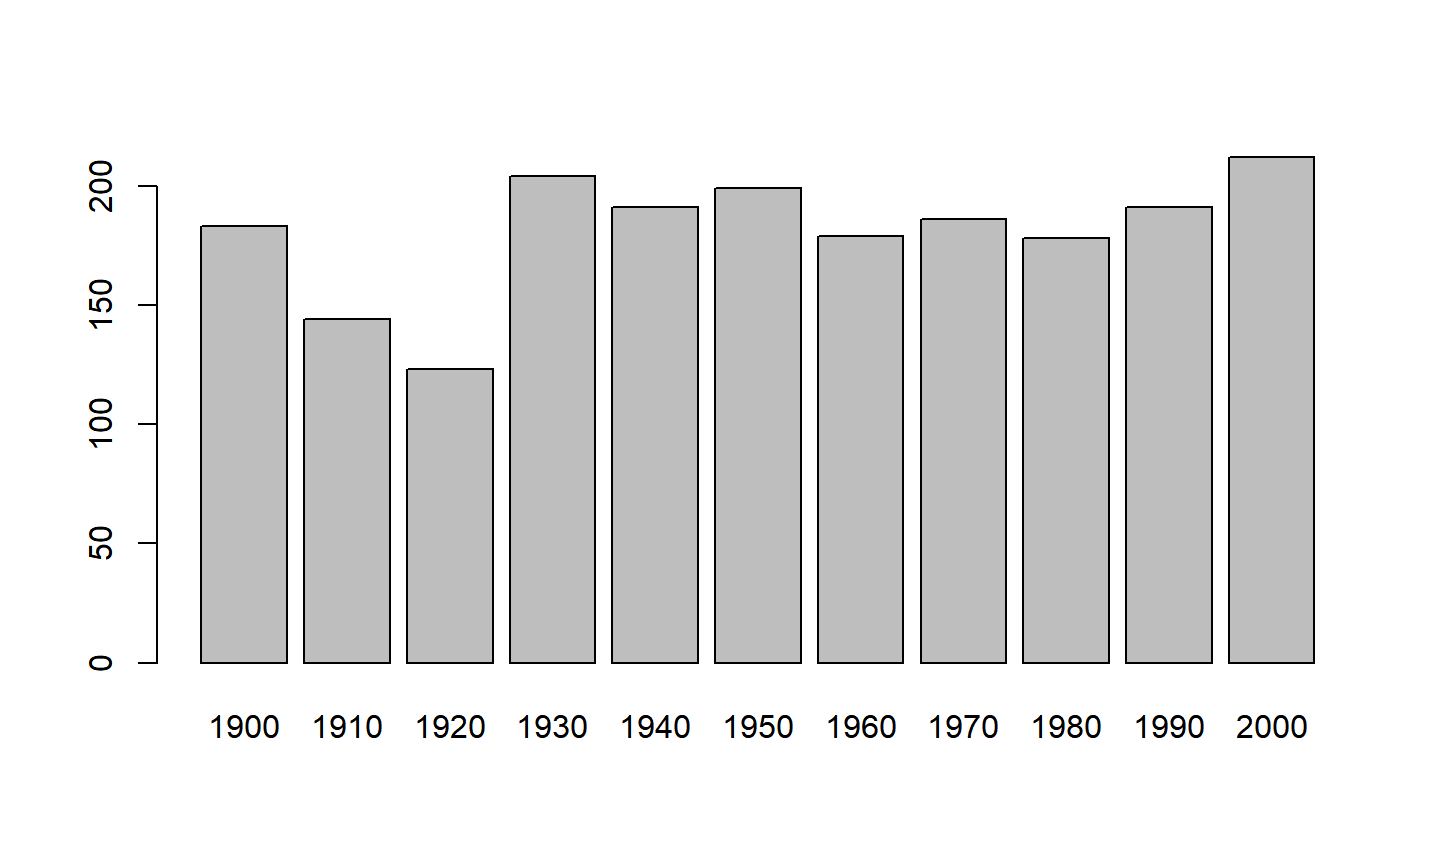
\includegraphics[width=0.7\linewidth]{lista-06-resolucao_files/figure-latex/unnamed-chunk-6-1} \end{center}

\hypertarget{seguros-mais-calculos}{%
\subsection{Seguros: mais cálculos}\label{seguros-mais-calculos}}

\hypertarget{exercicio-5}{%
\subsubsection{Exercício 5}\label{exercicio-5}}

\begin{Shaded}
\begin{Highlighting}[]
\NormalTok{VPA =}\StringTok{ }\DecValTok{1000}\OperatorTok{*}\DecValTok{12}\OperatorTok{*}\NormalTok{( }\KeywordTok{axn}\NormalTok{(soa08Act, }\DataTypeTok{x=}\DecValTok{30}\NormalTok{, }\DataTypeTok{k=}\DecValTok{12}\NormalTok{) }\OperatorTok{-}\StringTok{ }\KeywordTok{axyzn}\NormalTok{(}\KeywordTok{list}\NormalTok{(soa08Act, soa08Act), }\DataTypeTok{x=}\KeywordTok{c}\NormalTok{(}\DecValTok{30}\NormalTok{,}\DecValTok{40}\NormalTok{), }\DataTypeTok{k=}\DecValTok{12}\NormalTok{) )}
\NormalTok{P =}\StringTok{ }\NormalTok{VPA}\OperatorTok{/}\NormalTok{(}\DecValTok{12}\OperatorTok{*}\KeywordTok{axyzn}\NormalTok{(}\KeywordTok{list}\NormalTok{(soa08Act,soa08Act),}\KeywordTok{c}\NormalTok{(}\DecValTok{30}\NormalTok{,}\DecValTok{40}\NormalTok{),}\DataTypeTok{n=}\DecValTok{30}\NormalTok{,}\DataTypeTok{k=}\DecValTok{12}\NormalTok{))}
\end{Highlighting}
\end{Shaded}

\textbf{a)} O VPA da anuidade reversível é \$19801.1.

\textbf{b)} O prêmio mensal para esse contrato é \$127.06.

\hypertarget{exercicio-6}{%
\subsubsection{Exercício 6}\label{exercicio-6}}

\begin{Shaded}
\begin{Highlighting}[]
\NormalTok{G =}\StringTok{ }\NormalTok{(}\DecValTok{10000}\OperatorTok{*}\KeywordTok{Axn}\NormalTok{(soa08Act,}\DecValTok{30}\NormalTok{,}\DecValTok{20}\NormalTok{)}\OperatorTok{+}\DecValTok{30}\OperatorTok{*}\KeywordTok{axn}\NormalTok{(soa08Act,}\DecValTok{30}\NormalTok{,}\DecValTok{20}\NormalTok{))}\OperatorTok{/}\NormalTok{(}\FloatTok{0.85}\OperatorTok{*}\KeywordTok{axn}\NormalTok{(soa08Act,}\DecValTok{30}\NormalTok{,}\DecValTok{20}\NormalTok{))}
\end{Highlighting}
\end{Shaded}

O prêmio bruto para esse contrato é \$64.15.

\hypertarget{exercicio-7}{%
\subsubsection{Exercício 7}\label{exercicio-7}}

Uma amostra de \(K_{25}\) pode ser gerada com o seguinte comando:

\begin{Shaded}
\begin{Highlighting}[]
\NormalTok{K25 =}\StringTok{ }\KeywordTok{rLife}\NormalTok{(}\DataTypeTok{n=}\DecValTok{10}\OperatorTok{^}\DecValTok{4}\NormalTok{, }\DataTypeTok{object=}\NormalTok{soa08Act, }\DataTypeTok{x=}\DecValTok{25}\NormalTok{, }\DataTypeTok{type=}\StringTok{"Kx"}\NormalTok{)}
\end{Highlighting}
\end{Shaded}

\textbf{a)} As estatísticas descritivas e o histograma da amostra de
\(K_{25}\) podem ser vistos abaixo.

\begin{verbatim}
##    Min. 1st Qu.  Median    Mean 3rd Qu.    Max. 
##    0.00   42.00   52.00   49.32   59.00   78.00
\end{verbatim}

\begin{center}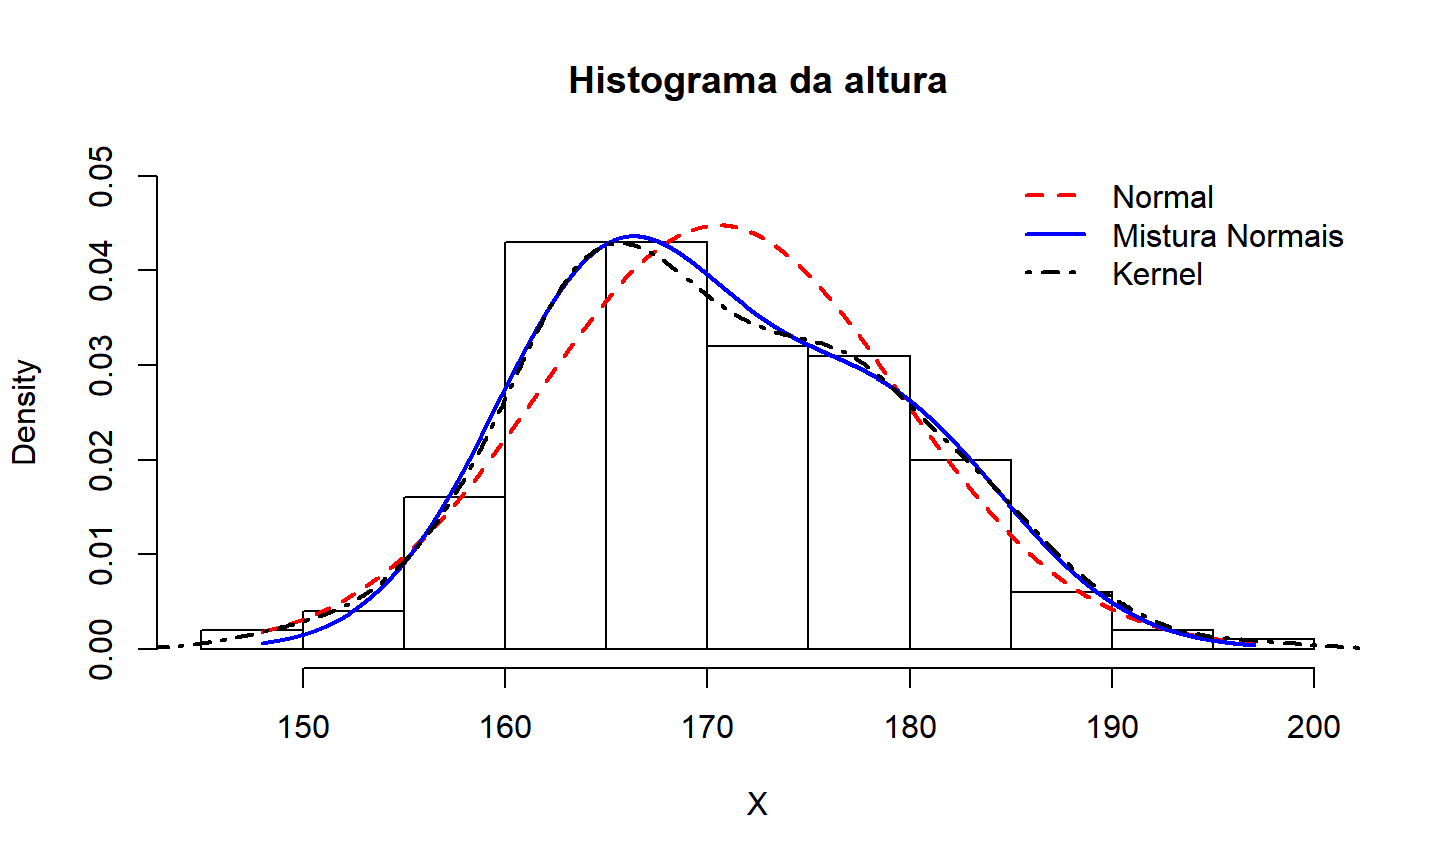
\includegraphics[width=0.7\linewidth]{lista-06-resolucao_files/figure-latex/unnamed-chunk-11-1} \end{center}

\textbf{b)} Podemos estimar a probabilidade de um indivíduo de 25 anos
sobreviver até os 60 anos usando a amostra simulada acima. Como vemos
abaixo, a probabilidade estimada é bem próxima da probabilidade teórica
obtida a partir da tábua de mortalidade.

\begin{Shaded}
\begin{Highlighting}[]
\NormalTok{## probabilidade estimada}
\KeywordTok{mean}\NormalTok{(K25}\OperatorTok{>}\DecValTok{35}\NormalTok{)}
\end{Highlighting}
\end{Shaded}

\begin{verbatim}
## [1] 0.8436
\end{verbatim}

\begin{Shaded}
\begin{Highlighting}[]
\NormalTok{## probabilidade teórica}
\KeywordTok{pxt}\NormalTok{(soa08Act, }\DataTypeTok{x=}\DecValTok{25}\NormalTok{, }\DataTypeTok{t=}\DecValTok{35}\NormalTok{)}
\end{Highlighting}
\end{Shaded}

\begin{verbatim}
## [1] 0.8560439
\end{verbatim}

\hypertarget{exercicio-8}{%
\subsubsection{Exercício 8}\label{exercicio-8}}

\begin{Shaded}
\begin{Highlighting}[]
\NormalTok{a65 =}\StringTok{ }\DecValTok{1000}\OperatorTok{*}\KeywordTok{rLifeContingencies}\NormalTok{(}\DataTypeTok{n=}\DecValTok{100000}\NormalTok{, }\DataTypeTok{lifecontingency=}\StringTok{"axn"}\NormalTok{, }\DataTypeTok{object=}\NormalTok{soa08Act,}
                              \DataTypeTok{x=}\DecValTok{65}\NormalTok{, }\DataTypeTok{parallel=}\OtherTok{TRUE}\NormalTok{)}
\NormalTok{P.perc =}\StringTok{ }\KeywordTok{quantile}\NormalTok{(a65, }\DataTypeTok{p=}\FloatTok{0.75}\NormalTok{)}
\end{Highlighting}
\end{Shaded}

O prêmio para esse contrato obtido de acordo com o princípio do
percentil é \$12764.08.


\end{document}
